\documentclass{article}

\usepackage[fleqn]{amsmath}
\usepackage{amssymb}
\usepackage{hyperref}
\usepackage{url}
\usepackage{graphicx}
\usepackage{geometry}
\usepackage{babel}
\usepackage{enumitem}
\usepackage{parskip}
\usepackage{chemfig}
\usepackage{pdfpages}
\usepackage{xcolor}
\usepackage{tikz}
\usepackage{fancybox}
\usepackage{makecell}
\usepackage{pgfplots}
\usepackage{soul}
\usepackage{ulem}
\usepackage{wrapfig}
\usepackage{subcaption}
\usepackage[T1]{fontenc}
\usepackage{esvect}
\usetikzlibrary{arrows}
\usetikzlibrary{decorations.pathreplacing}
\pgfplotsset{compat=1.17}

\geometry{
    a4paper,
    total={170mm, 257mm},
    left=20mm,
    top=20mm
}

\hypersetup{
    colorlinks=true,
    linkcolor=black,
    urlcolor=blue,
    pdftitle={Basis of Sustainable Environmental Systems}
}

\newcommand{\figbox}[1]{ 
    \begin{figure*}[ht!]        
        \begin{center}            
            \fbox{#1}        
        \end{center}    
    \end{figure*}
}

\newcommand{\wrapfill}{
    \par
    \ifnum \value{WF@wrappedlines} > 0
        \addtocounter{WF@wrappedlines}{-1}%
        \null\vspace{
            \arabic{WF@wrappedlines}
            \baselineskip
        }
        \WFclear
    \fi
    \phantom{}
}

\newcommand{\cfig}[1]{%
  \begin{figure*}[ht!]%
    \centering%
    #1%
  \end{figure*}%
}

\newcommand{\difference}{\,\backslash\,}
\newcommand{\rem}{\underline{Remark}: }
\newcommand{\nots}{\underline{Notation}: }
\newcommand{\prf}{\underline{Proof}: }
\newcommand{\exs}{\underline{Example}: }
\newcommand{\defs}{\underline{Definition}: }
\newcommand{\wrn}{\underline{Warning}: }
\newcommand{\sht}{\ |\ }
\newcommand{\pph}[1]{\paragraph{#1}\phantom{}\\}


% === TEXT ===
\title{\textbf{Basis of Sustainable Environmental Systems \\ HSLU, Semester 3}}
\author{Matteo Frongillo}

\begin{document}

\maketitle
\tableofcontents
\pagebreak

\part{TODO ops}
i'll do it later don't worry

\newpage
\part{Separation techniques}
\section{A bit of chem again}
\subsection{Solutions key terms}
\begin{itemize}
    \item \textbf{Solvent}: the substance that dissolves another substance 
    \item \textbf{Solute}: the substance that is dissolved in a solvent
    \item \textbf{Solution}: it's a homogeneous mixture of two or more substances
\end{itemize}

What it is needed?
\begin{itemize}
    \item Identify the substances to be separated from the mixture
    \item To collect useful substances free from impurities
    \item To remove unwanted particles
\end{itemize}

\subsection{Classification of techniques}
\begin{figure*}[ht!]
    \centering
    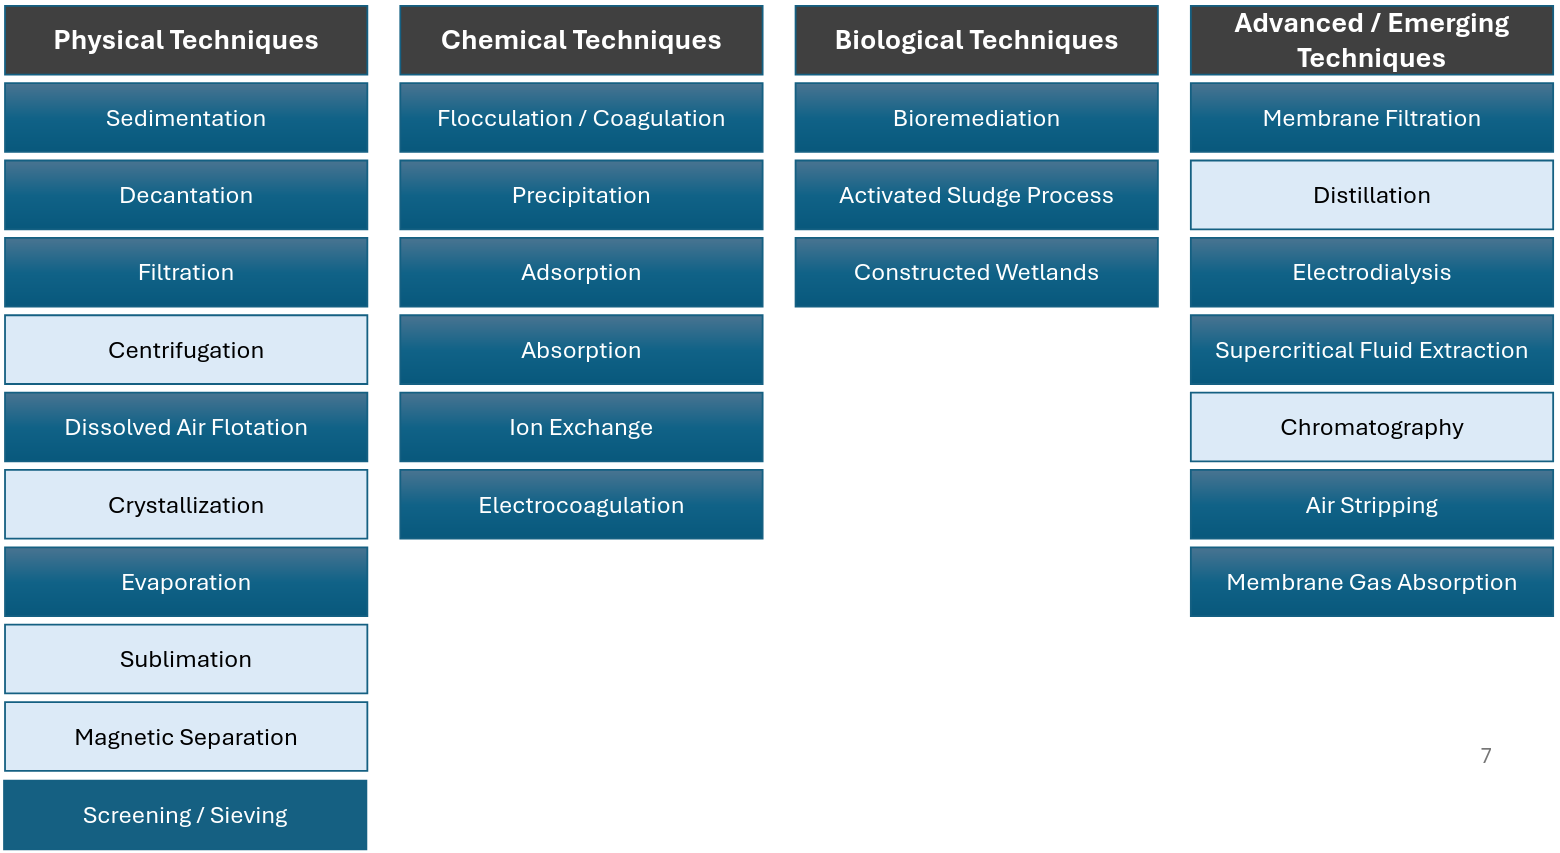
\includegraphics[width=\textwidth]{media/techniques_overview.png}
    \caption*{Separation techniques overview}
\end{figure*}

\section{Physical separation}
\subsection{Sedimentation}

\subsection{Decantation}

\subsection{Filtration}

\subsubsection{Sand filtration}

\subsubsection{Reverse osmosis}

\subsection{Centrifugation}

\subsection{Dissolved Air Flotation (DAF)}

\subsection{Magnetic separation}

\subsection{Screening and Sieving}

\newpage
\section{Chemical separation}

\subsection{Flocculation}
\subsubsection{Flocculant}

\subsubsection{Coagulation}

\subsection{Electrocoagulation}

\subsection{Precipitation}

\subsection{Adsorbtion}

\subsubsection{Activated carbon}

\subsection{Absorption}

\subsubsection{Wet scrubber}

\subsection{Ion exchange}

\subsection{Crystallization}

\subsection{Evaporation}

\subsection{Sublimation}

\newpage
\section{Advanced/Emerging separation}

\subsection{Mebrane filtration}

\subsubsection{Micro osmosis}

\subsubsection{Nano osmosis}

\subsubsection{Ultra osmosis}

\subsubsection{Reverse osmosis}

\subsection{Electrodialysis}

\subsection{Extraction}

\subsubsection{Liquid-Liquid Extraction (LLE)}

\subsubsection{Soxhlet extraction}

\subsubsection{Supercritical Fluid Extraction}

\subsection{Air stripping}
Same as Wet Scrubber, but with water

\subsection{Electrostatic precipitator (ESP)}














\end{document}
